\documentclass[dvipsnames,beamer]{standalone}

\usepackage{tikz}
\usetikzlibrary{positioning,decorations.pathreplacing,fit}
\usetikzlibrary{decorations.markings,arrows.meta,shapes.arrows}
\usetikzlibrary{calc}

\definecolor{mygreen}{RGB}{0,128,80}
\colorlet{darkgreen}{mygreen!90!black}


\begin{document}

%\small


\begin{standaloneframe}

\resizebox{\textwidth}{!}{

\begin{tikzpicture}[
	arrow double line/.style={
		double distance = 20pt,
   		shorten <= 11, 	
   		shorten >= 16,
   		very thick,
	    postaction = {
    		draw = white,
	 	    line width = 20pt,
	 	    shorten <=-.1pt,
	 	    shorten >=-.1pt,	
	    },
	    postaction = {
	    	decorate, 
	    	decoration = {
	    		markings, 
	    		mark=at position 0 with {
	    			\arrow[xshift=26.6pt]{Straight Barb[reversed,length=-1pt 0.7]}
	    		},
	    		mark = at position 1 with {
   	    			\arrow[xshift=10.6pt]{Straight Barb[length=-1pt 0.7]}
   	    		}
	    	}
	    }
	},
	fat arrow double line/.style={
		double distance = 23pt,
   		shorten <= 12.5, 	
   		shorten >= 17.5,
   		very thick,
		 postaction = {
		   		draw = white,
		  line width = 23pt,
		  shorten <=-.1pt,
		  shorten >=-.1pt,	
		 },
		 postaction = {
	    	decorate, 
	    	decoration = {
	    		markings, 
	    		mark=at position 0 with {
	    			\arrow[xshift=29.4pt]{Straight Barb[reversed,length=-3pt 0.75]}
	    		},
	    		mark = at position 1 with {
	  	    			\arrow[xshift=12.6pt]{Straight Barb[length=-3pt 0.75]}
	  	    		}
	    	}
 		}
	},
	mysingle/.style = {
		double distance = 27,
		shorten <= 8.8, 	
		shorten >= 14,
		very thick,
		postaction = {
	 		draw = white,
			line width = 27pt,
			shorten <=8pt,
			shorten >=-.5pt,	
		},
		postaction = {
			decorate, 
			decoration = {
				markings, 
				mark = at position 1 with {
					\arrow [xshift=21]{Straight Barb[length=-4pt 0.75]}
				}
			}
		},	
	},
	mybrace/.style= {
		decorate, decoration={brace,amplitude=5pt,raise=5pt}, thick
	},
	every node/.style={
		font=\bfseries
	},	
	]

	

		
	\node[] (client) {Client};
	\node[right = 4.4 of client] (AP) {Authenticator};
	\node[right = 4.1 of  AP] (AS) {Server};
	\def\InterMsgSpaceVertical{1.2}
	

	\node[inner sep=0pt, xshift=0cm,yshift=0.8cm] (laptop_icon) at (client) {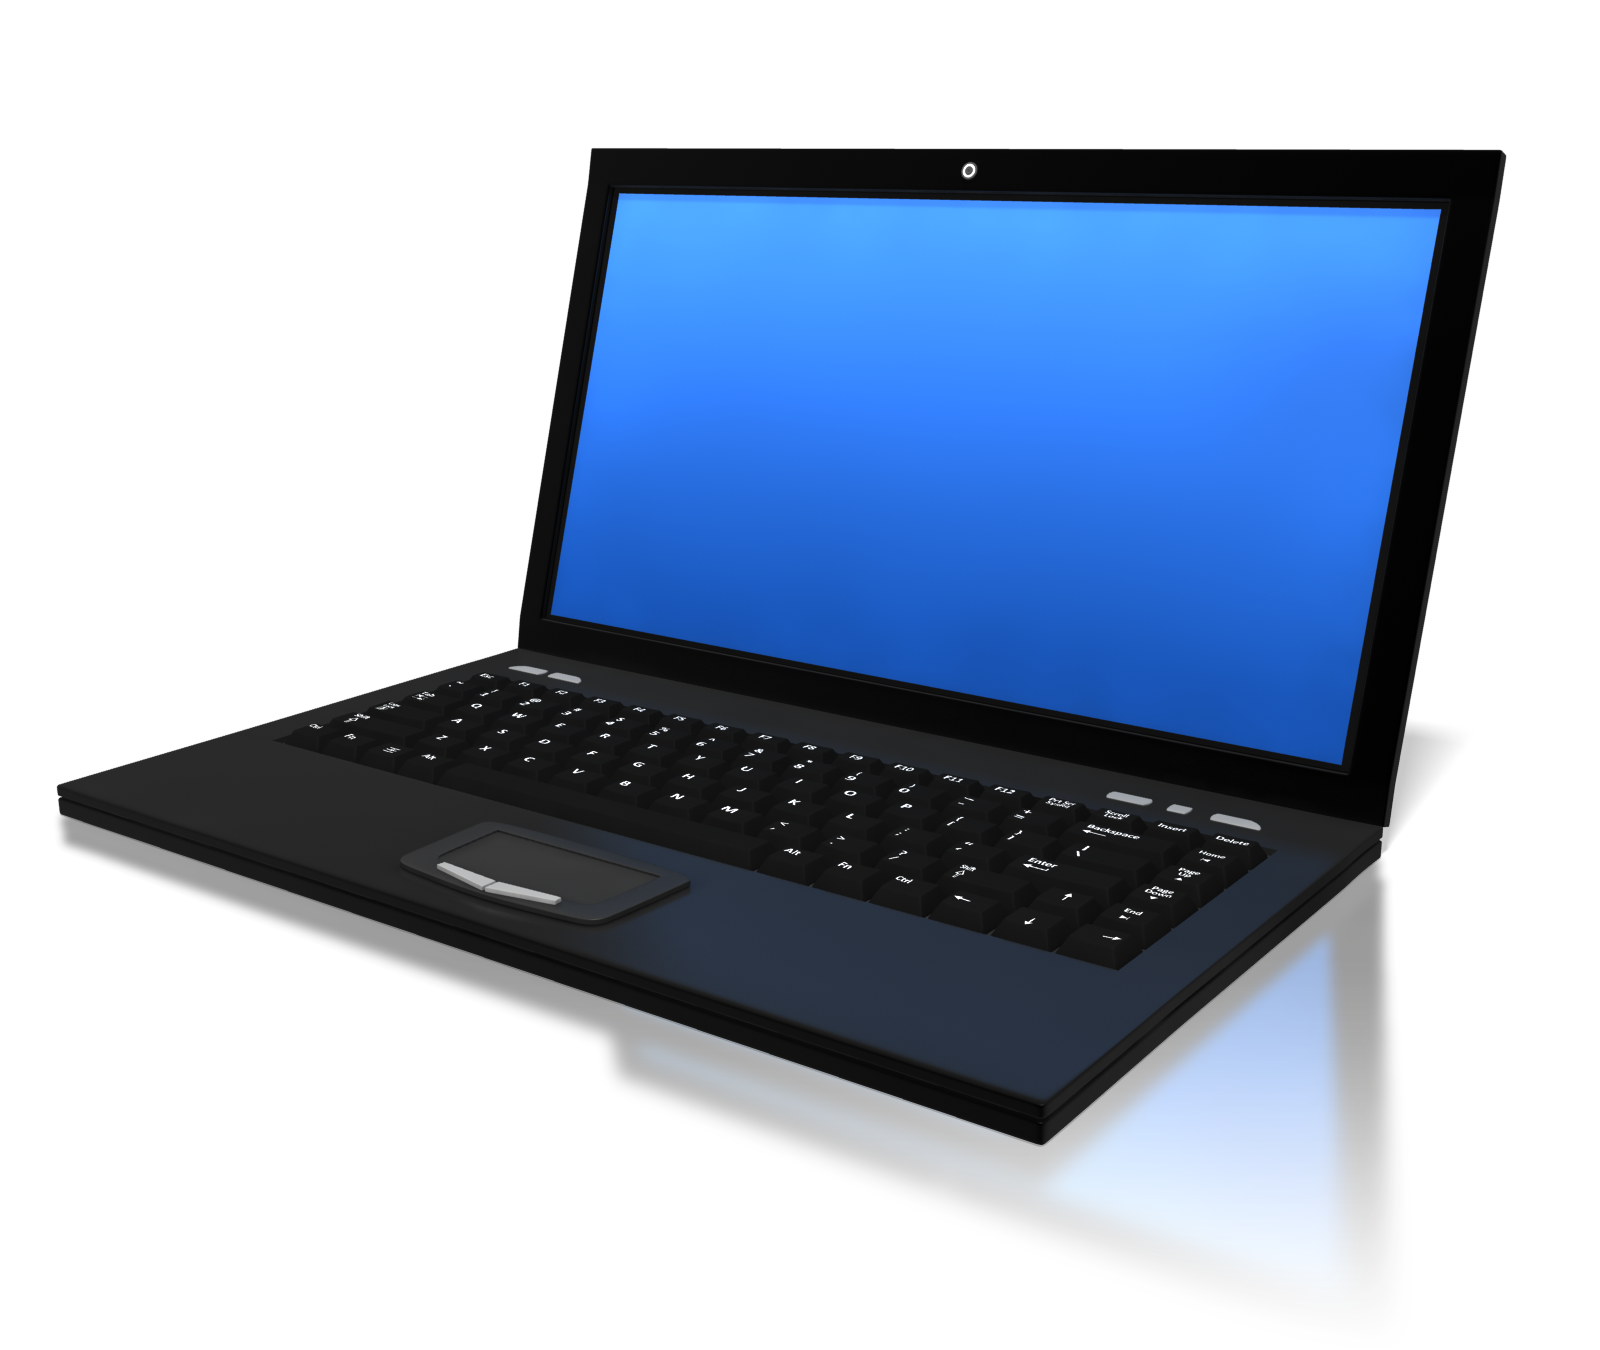
\includegraphics[width=.15\textwidth]{laptop}};
	
	\node[inner sep=0pt, xshift=-0.0cm,yshift=1.1cm] (AP_icon) at (AP) {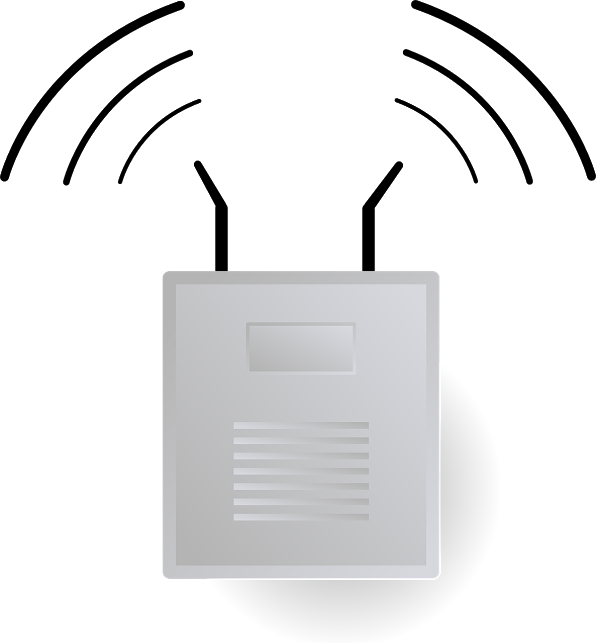
\includegraphics[width=.13\textwidth]{AP}};


	\node[above = -0.2 of AS] () {
\includegraphics[width=.1\textwidth]{server}};

	
	\foreach \i in {1,...,3} {%
		\coordinate[below = \InterMsgSpaceVertical * \i of client] (c\i) {};
		\coordinate[below = \InterMsgSpaceVertical * \i of AP] (ap\i) {};
		\coordinate[below = \InterMsgSpaceVertical * \i of AS] (as\i) {};
	}	
	\visible<1-4>{%
		\draw[arrow double line,red] (c1) -- node (EAP) {EAP method (EAP-TLS)} (as1);
		\draw[arrow double line,blue] (ap2) -- node[xshift=-2] (AAA) {Key-transport (RADIUS)} (as2);
	}	
	\visible<2-3>{%
		\draw[arrow double line,darkgreen] (c3) -- node[xshift=-2] {IEEE 802.11} (ap3);
	}	
	\visible<3>{%
		\draw[mybrace] ([yshift=15]as1) -- node[right=0.4,align=center] (3P-KD) {EAP} ([yshift=-15]as2);
		\draw[mybrace, decoration={mirror}, left] ([yshift=15]c1) -- node[left=0.4,align=center] {WPA2\\Enterprise} ([yshift=-15]c3);
	}	
	\visible<4-5>{%
		\draw[arrow double line,darkgreen] (c3) -- node[xshift=-2] {Key-confirmation} (ap3);
	}
	\visible<5>{%
		\draw[fat arrow double line, Plum] (c1) -- node[xshift=5pt] {EAP} (as1);
		\draw[mysingle, Plum] ([yshift=-3]ap1) --  ([yshift=-4]ap2);
	}
\end{tikzpicture}

}
\end{standaloneframe}


\end{document}